% Author: Till Tantau
% Source: The PGF/TikZ manual
%\documentclass{minimal}
\documentclass[tikz,border=2mm]{standalone}
\usepackage{tikz}
%\usetikzlibrary{trees,snakes}
\usepackage{verbatim}

\usepackage{tkz-euclide}
\usetkzobj{all}


\usetikzlibrary{backgrounds,angles,quotes}

\begin{document}
\pagestyle{empty}

\begin{comment}
:Title: A picture for Karl's students
:Slug: tutorial
:Tags: Manual

This example is from the tutorial: A picture for Karl's students.

| Author: Till Tantau
| Source: The PGF/TikZ manual


\end{comment}

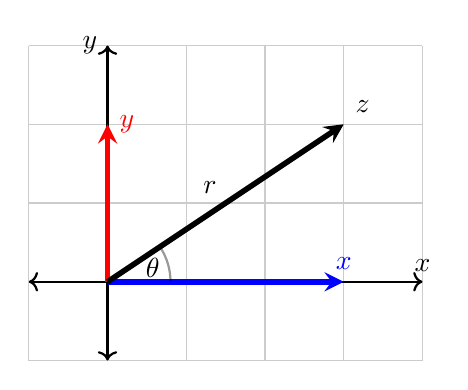
\begin{tikzpicture} [thick]
  \draw[thin,gray!40] (-1,-1) grid (4.0,3.0);
  \draw[<->] (-1,0)--(4,0) node[above]{$x$};
  \draw[<->] (0,-1)--(0,3) node[left]{$y$};
  \draw[line width=2pt,blue,-stealth](0,0)--(3,0) node[above]{$x$};
  \draw[line width=2pt,red,-stealth](0,0)--(0,2) node[right]{$y$};
  \draw[line width=2pt,black,-stealth](0,0)--(3,2) node[anchor=south west]{$z$};
  \node[] at (1.3,1.2) {$r$};


\coordinate (O) at (0,0);
\coordinate (A) at (3,0);
\coordinate (B) at (3,2);
%\draw (O)--(A)--(B)--cycle;

\tkzMarkAngle[fill= orange,size=0.8cm,opacity=.4](A,O,B)
\tkzLabelAngle[pos = 0.6](A,O,B){$\theta$}

%\shade[inner color = black, outer color = blue] (0,0) circle (0.1);
%\shade[inner color = black, outer color = red] (5,5) circle (0.1);

\end{tikzpicture}

\end{document}